Le monde d’IoT représente par définition un système “intégré”, où les différents objets interagissent entre eux, sont inter-connectés, à travers l’échange d’informations et de commande (requête, demande). Ces objets ont une forte probabilité d’être hétérogènes en termes de niveau de sécurité, de privacité minimal garanti, de technologie, de protocole de communication, et de politique d’exécution. Le challenge est ainsi davantage lié au besoin d’avoir une structure horizontale capable de gérer les spécifications de sécurité et de privacité de manière unique et homogène. Ces spécifications auront besoin en effet d’être instanciées sur des “entités” et auront potentiellement des interfaces d’implémentation, de spécification et de communication différentes.
\\

Les caractéristiques de IoT comprennent donc un réseau à très grande échelle des objets, une grande hétérogénéité au niveau des dispositifs et du réseau, et un grand nombre d'événements générés spontanément par ces objets. Malheureusement, toutes ces caractéristiques feront du développement des diverses applications et des services une tâche très difficile. En général, le middleware peut faciliter un processus de développement en intégrant des dispositifs informatiques et de communication hétérogènes, et en soutenant l'interopérabilité au sein des diverses applications et services.

En effet, un middleware fait abstraction de la complexité du système ou du matériel, permettant au développeur d'applications de concentrer tous ses efforts sur la tâche à résoudre, sans la distraction des préoccupations orthogonales au niveau du système ou du matériel. Ces complexités peuvent être liées à des préoccupations de communication ou au calcul plus généralement. Un middleware fournit une couche logicielle entre les applications, le système d'exploitation, les couches de communication réseau et les différents dispositifs du système, ce qui facilite et coordonne certains aspects du traitement coopératif. Du point de vue informatique, un middleware fournit une couche entre les logiciels d'application et des logiciels système. Dans l'IoT, l’hétérogénéité des dispositifs implique très souvent une hétérogénéité considérable dans les technologies de communication utilisées, ainsi que dans les technologies au niveau du système, c’est pourquoi un middleware devrait supporter ces deux types d’hétérogénéité. Nous avons donc besoin d’un middleware qui respecte des caractéristiques, que nous décrirons par des modules. Ces modules seront divisés en trois groupes : les modules fonctionnels, liés aux services et aux fonctions que notre middleware doit fournir ; les modules non-fonctionnels, liés à la Quality of Service (QoS), aux performances et aux différentes exigences que notre middleware devra prendre en compte; et les modules architecturaux, liés à l’architecture de notre middleware.
\\
\begin{figure}[h!]
	\hspace*{-1cm}
	\centering
	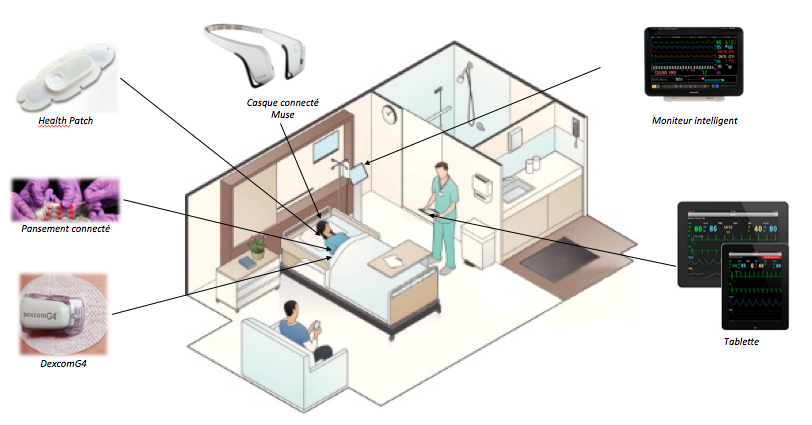
\includegraphics[width=1.1\textwidth]{Figure1.png}
	\caption{Couches Dispositifs, et Protocoles de Réseau et de Communication de notre Système}
	\label{fig:balance}
\end{figure}

Rappelons que notre sujet consiste à établir un système IoT dans le domaine Smart Health, et plus précisément dans les services de soins intensifs des hôpitaux, afin de résoudre le problèmes de congestion et de surveillance en continu dans ces services. La Figure 1 nous permet de visualiser les choix de dispositifs et de protocoles de communication et de réseau que nous avons établis dans le rapport précédent. Avant de commencer à décrire les différents modules dont nous auront besoin dans notre middleware, ce que nous feront dans les section 2, 3, et 4, il est important de préciser le choix que nous avons fait concernant l’architecture générale de notre middleware. En effet, nous avons décidé de diviser notre middleware en deux couches différentes, la première étant liée au moniteur qui centralise toutes les informations des divers dispositifs présents dans la chambre du patient, et qui donc va gérer l’hétérogénéité entre les dispositifs présents dans l’environnement du patient. La seconde couche middleware est liée au Gateway de notre système, qui s’occupe de centraliser les informations de tous les moniteurs (le problème d’hétérogénéité se pose moins ici), et qui va faire le lien entre la couche de stockage et celle de liaison à la couche physique. Cette seconde couche va être celle qui permettra d’identifier les différents groupements de dispositifs à travers la connaissance des différents moniteurs intelligents.

La Figure 2 nous permet de visualiser la structure de notre système en considérant seulement les couches dispositifs, réseaux et communication, middleware, et architecture. Ainsi, dans les trois prochaines sections, notre tâche ne sera pas seulement de décrire les différents modules dont nous avons besoin dans notre middleware, mais aussi de décrire dans quelle(s) couche(s) middleware nous en avons besoin (possiblement les deux).

\begin{figure}[h!]
	\hspace*{-2.5cm}
	\centering
	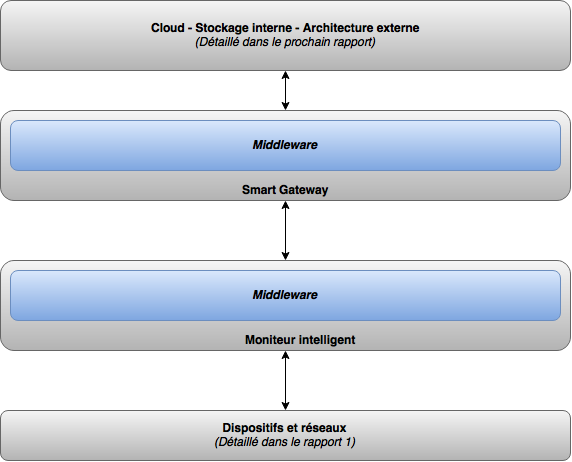
\includegraphics[width=1.4\textwidth]{Figure2.png}
	\caption{Vue Globale de notre Middleware au sein de notre Système}
	\label{fig:balance}
\end{figure}
